%**********
% Preamble
%**********
\pdfoutput=1
%\pdfoutput=1
\PassOptionsToPackage{usenames,dvipsnames}{xcolor}
\iffalse
\documentclass[10pt]{article}
\fi
%\usepackage{helvet}
%\renewcommand{\familydefault}{\sfdefault}
\iftrue 
\documentclass[11pt]{SelfArx}
\definecolor{color1}{HTML}{81071c} %   0,0,90  Color of the article title and sections
\definecolor{color2}{RGB}{0.972549,0.8352941, 0.5137255} % Color of the boxes behind the abstract and headings
\definecolor{light-gray}{gray}{0.05}
\color{light-gray}
\JournalInfo{\today} % Journal information
\Archive{XXXX} % Additional notes (e.g. copyright, DOI, review/research article)
\PaperTitle{
 Facilities, Equipment, and Other Resources
} % Article title
\Authors{
}
\Keywords{} % Keywords - if you don't want any simply remove all the text between the curly brackets
\newcommand{\keywordname}{Keywords} % Defines the keywords heading name
\Abstract{}
\fi

%\usepackage{helvet}
%\renewcommand{\familydefault}{\sfdefault}
%\usepackage[T1]{fontenc}
%\usepackage{courier} 
%\usepackage{fontspec}
%\setmainfont{Arial}
\usepackage[margin=1in]{geometry}
\usepackage[normalem]{ulem}\normalem
\usepackage{epsfig,ifthen}
\usepackage{color}
\usepackage{boxedminipage}
\usepackage{amsfonts}
\usepackage{amsmath}
\usepackage{amsthm}
\usepackage{url}
%\usepackage[hmargin=1in,vmargin=1in]{geometry}
\usepackage{enumitem}
%\usepackage{natbib}
\usepackage{pdfpages}
\usepackage{cancel}
\usepackage[colorinlistoftodos,bordercolor=orange,backgroundcolor=orange!20,linecolor=orange,textsize=scriptsize]{todonotes}
%\setlength{\bibsep}{0pt plus 0.3ex}
%\setlength{\columnsep}{0.55cm} % Distance between the two columns of text
%\setlength{\fboxrule}{0.75pt} % Width of the border around the abstract
%----------------------------------------------------------------------------------------
%	COLORS
%----------------------------------------------------------------------------------------
%	HYPERLINKS
%----------------------------------------------------------------------------------------
\usepackage{hyperref} % Required for hyperlinks
\usepackage{wrapfig}
\iffalse
\usepackage{tikz}
\usetikzlibrary{backgrounds}
\makeatletter
\usepackage{epsfig}
\usepackage{color}
\usepackage{boxedminipage}
\usepackage{amsfonts}
\usepackage{amsmath}
\usepackage{url}
%\usepackage[hmargin=1in,vmargin=1in]{geometry}
\usepackage{enumitem}
\usepackage{natbib}
\usepackage{fec_styles/fec}
\usepackage{pdfpages}

\tikzset{%
  fancy quotes/.style={
    text width=\fq@width pt,
    align=justify,
    inner sep=1em,
    anchor=north west,
    minimum width=\linewidth,
  },
  fancy quotes width/.initial={.8\linewidth},
  fancy quotes marks/.style={
    scale=8,
    text=white,
    inner sep=0pt,
  },
  fancy quotes opening/.style={
    fancy quotes marks,
  },
  fancy quotes closing/.style={
    fancy quotes marks,
  },
  fancy quotes background/.style={
    show background rectangle,
    inner frame xsep=0pt,
    background rectangle/.style={
      fill=gray!25,
      rounded corners,
    },
  }
}

\newenvironment{fancyquotes}[1][]{%
\noindent
\tikzpicture[fancy quotes background]
\node[fancy quotes opening,anchor=north west] (fq@ul) at (0,0) {``};
\tikz@scan@one@point\pgfutil@firstofone(fq@ul.east)
\pgfmathsetmacro{\fq@width}{\linewidth - 2*\pgf@x}
\node[fancy quotes,#1] (fq@txt) at (fq@ul.north west) \bgroup}
{\egroup;
\node[overlay,fancy quotes closing,anchor=east] at (fq@txt.south east) {''};
\endtikzpicture}

\makeatother
\fi

\newtheorem{theorem}{Theorem}
\newtheorem{definition}[theorem]{Definition}
\newtheorem{lemma}[theorem]{Lemma}
\newtheorem{proposition}[theorem]{Proposition}
\newtheorem{corollary}[theorem]{Corollary}
\newtheorem{remark}[theorem]{Remark}
\newtheorem{example}[theorem]{Example}
\newtheorem{assumption}[theorem]{Assumption}
\DeclareMathOperator{\sgn}{sgn}
\DeclareMathOperator{\Rand}{Rand}
\DeclareMathOperator{\support}{support}
\DeclareMathOperator{\Diag}{Diag}
\DeclareMathOperator{\diam}{diam}
\DeclareMathOperator{\dom}{dom}         % domain
\DeclareMathOperator*{\argmin}{arg\,min}
\DeclareMathOperator*{\argmax}{arg\,max}

\newcommand{\del}[1]{{\color{red}#1}}            % comment
\newcommand{\st}{\;:\;}                          % such that
\newcommand{\ve}[2]{\left\langle #1 ,  #2 \right\rangle}    % inner product
\newcommand{\eqdef}{:=}
\newcommand{\R}{\mathbb{R}}                      % set of real numbers
\newcommand{\Prob}{\mathbb{P}}                   % probability
\newcommand{\E}{\mathbb{E}}                      % expectation
\newcommand{\N}{n}                               % dimension of the problem =N; there will be n<=N blocks
\newcommand{\U}{U}
\newcommand{\C}{\mathcal{C}}

\newcommand{\diag}{\mathbf{diag}}
\newcommand{\Var}{\mathbf{Var}}
\newcommand{\hatZ}{\hat Z}
\newcommand{\hatS}{\hat S}
\newcommand{\calG}{G}
\newcommand{\calT}{\mathcal{T}}
\newcommand{\calF}{\mathcal{F}}
\newcommand{\Lip}{\mathcal{L}}
\newcommand{\calH}{\mathcal{H}_\beta}
\newcommand{\calHMINI}{\mathcal{C}}

\newcommand{\calS}{\mathcal{S}}
\newcommand{\calJ}{\mathcal{J}}
\renewcommand{\d}{ {\Delta}}
\newcommand{\x}{ {\bf x}}
\newcommand{\y}{ {\bf y}}
\newcommand{\z}{ {\bf z}}
\newcommand{\vv}{ {\bf v}}
\newcommand{\wv}{ {\bf w}}
\newcommand{\av}{ {\bf \alpha}}
\newcommand{\bv}{ {\bf \alpha}}
\newcommand{\V}{ {\bf v}}
\newcommand{\T}{ {\bf T}}
\newcommand{\X}{ {\bf X}}
\newcommand{\Q}{ {\bf Q}}
\newcommand{\0}{ {\bf 0}}
\newcommand{\alf}{ {\boldsymbol \alpha}}
\newcommand{\vchi}{ {\boldsymbol \chi}}

\newcommand{\vu}{{\bf u}}
\newcommand{\vdelta}{{\boldsymbol \delta} }
\newcommand{\w}{  {\bf w}}
\newcommand{\vt}{  {\bf t}}
\newcommand{\va}{  {\bf a}}
\renewcommand{\t}{{^\top}}

\newcommand{\f}{f}
\newcommand{\YY}{\varphi}
\newcommand{\K}{K}
\newcommand{\sK}{\mathcal{K}}
\newcommand{\J}{J}
\newcommand{\sJ}{\mathcal{J}}

\newcommand{\calO}{\mathcal{O}}
\newcommand{\vsubset}[2]{#1_{[#2]}}
\newcommand{\Srv}{\hat{S}}
\newcommand{\oo}{|J \cap \Srv_j|}

\newcommand{\vc}[2]{#1^{(#2)}}                   % coordinate of a vector
\newcommand{\cor}[2]{{{#1}_{#2}}}                   % coordinate of a vector
\newcommand{\corit}[3]{{#1}_{#2}^{(#3)}}                   % coordinate of a vector
\newcommand{\ncs}[2]{\|#1\|^2_{(#2)}}
\newcommand{\nbp}[2]{\|#1\|_{(#2)}}              % norm block primal
\newcommand{\nbd}[2]{\|#1\|_{(#2)}^*}            % norm block dual
\newcommand{\Rw}[2]{\mathcal R_{#1}(#2)}
\newcommand{\Rws}[2]{\mathcal R^2_{#1}(#2)}
\DeclareMathOperator{\trace}{trace}           % trace
\DeclareMathOperator{\card}{Card}           % Cardinality
\newcommand{\note}[1]{{\color{red} #1}}

\newcommand{\pnote}[1]{{  \color{red} [[ #1 -- Peter ]] }}
\newcommand{\natinote}[1]{{  \color{blue} [[ #1 -- Nati ]] }}
\newcommand{\takinote}[1]{{  \color{yellow} [[ #1 -- Martin ]] }}
\newcommand{\avnote}[1]{{  \color{green} [[ #1 -- Avleen ]] }}
\newcommand{\removed}[1]{}
\newcommand{\norm}[1]{\left\lVert{#1}\right\rVert}
\newcommand{\hingeloss}{\ell}
\newcommand{\hinge}[1]{\hingeloss ( #1 )}
\newcommand{\trans}{{\top}}
\newcommand{\calA}{\mathcal{A}}
\newcommand{\bP}{\mathcal{P}}
\newcommand{\bD}{\mathcal{D}}
\newcommand{\bH}{\mathcal{H}}
\newcommand{\sizeJ}{\omega}
\newcommand{\Gg}{\mathcal{G}^{\sigma'}}
\newcommand{\newstuff}[1]{{\color{red}#1}}
\newcommand{\cocoa}{\textsc{CoCoA}}
\newcommand{\cocoap}{\textsc{CoCoA$\!^{\bf \textbf{\footnotesize+}}$}}
\newcommand{\localalgname}{\textsc{LocalSolver}\xspace}
\newcommand{\localSDCA}{\textsc{LocalSDCA}\xspace}
\newcommand{\setn}{[n]}
\newcommand{\Exp}{\mathbb{E}}                      % expectation
\newcommand\tagthis{\addtocounter{equation}{1}\tag{\theequation}}

% For algorithms
\usepackage{algorithm}
\usepackage{algorithmic}
\usepackage{subfigure}

\newcommand{\rr}[1]{{\color{red}  #1 }}

% External referencing
%\usepackage{xcite}
%\externalcitedocument{../proposal/proposal}
\hypersetup{colorlinks,urlcolor=blue}

\let\oldFootnote\footnote
\newcommand\nextToken\relax

\renewcommand\footnote[1]{%
    \oldFootnote{#1}\futurelet\nextToken\isFootnote}

\newcommand\isFootnote{%
    \ifx\footnote\nextToken\textsuperscript{,}\fi}

%**********
% Document
%**********
\begin{document}
  
\begin{center}
  {\bf \large TRIPODS Institute for Optimization and Learning:}
  \smallskip
  
  {\bf \large Facilities, Equipment, and Other Resources}
\end{center} 
 

Lehigh has numerous facilities that can accommodate workshops and summer/winter schools.  The \href{https://lehighmountaintop.wordpress.com/learn-more/}{Mountaintop Campus} houses several such facilities
 that has been used by the Lehigh co-PIs and others in the past for 
events ranging from one day events to multiple day workshops. 

 \paragraph{The DISC Institute} In particular, the TRIPODS summer school in the summer of 2018 will be held in Building C in Mountaintop Campus which is the official location of the DISC institute. This facility, Lehigh's newest learning space on the Mountaintop campus, includes many modern features such as a telepresence
classroom and many teleconferencing and collaborative spaces for group projects (see pictures below).\\
\begin{center}
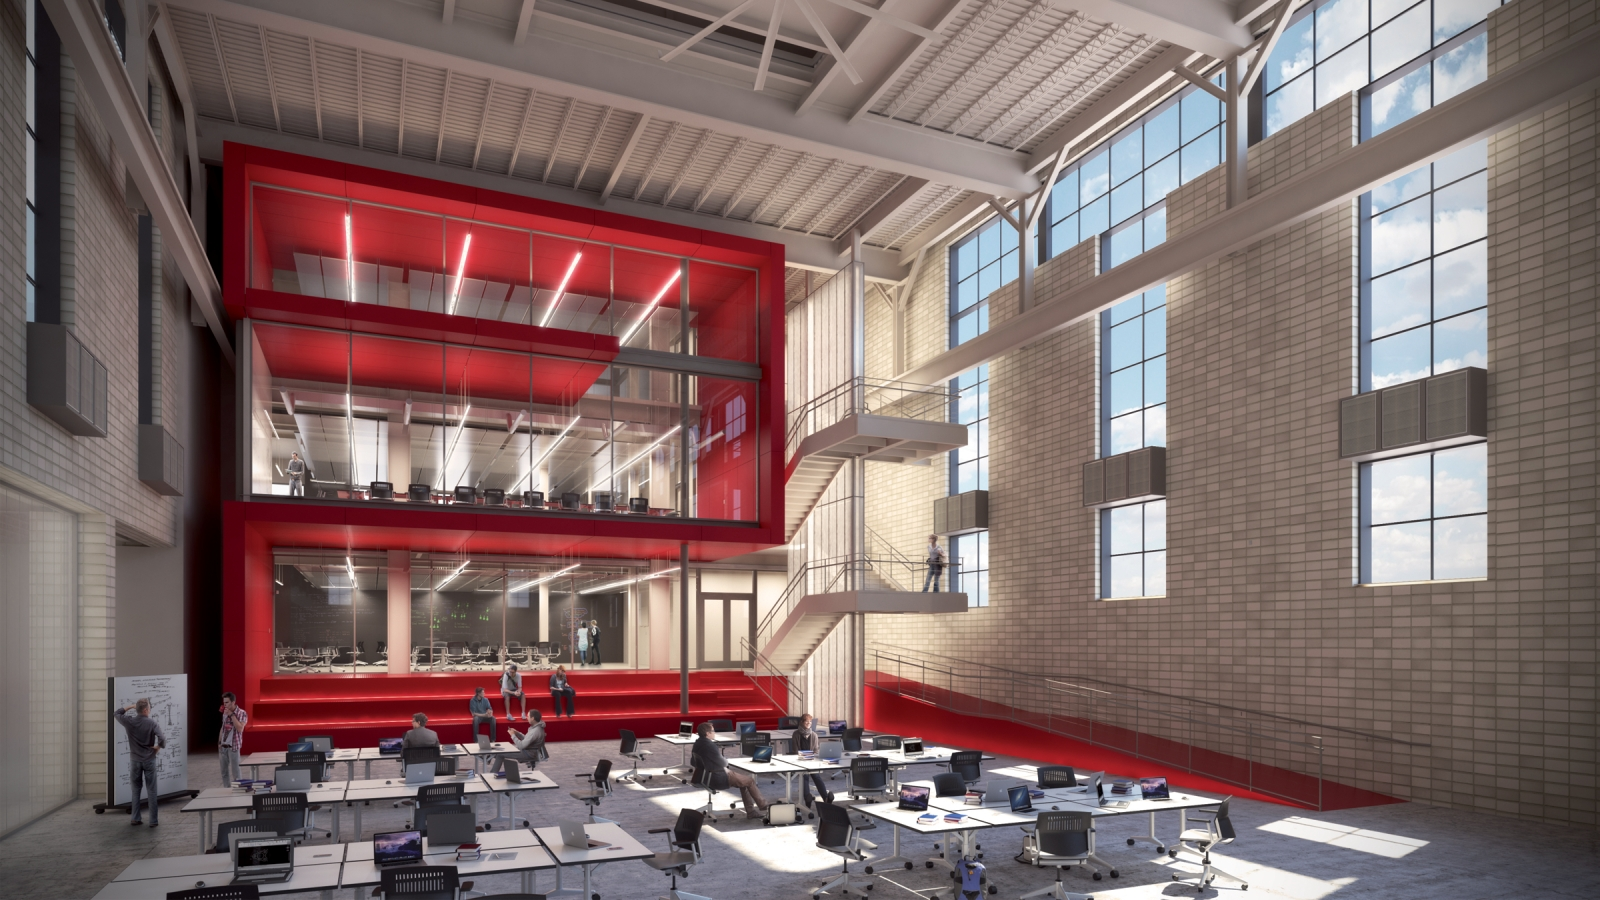
\includegraphics[height=3cm]{1012131_00_N5_bdc1_HERO.jpeg}
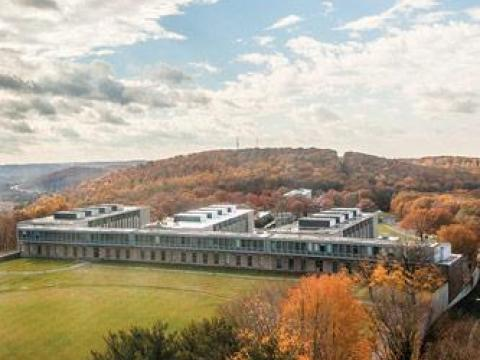
\includegraphics[height=3cm]{Mountaintop-BuildingC}
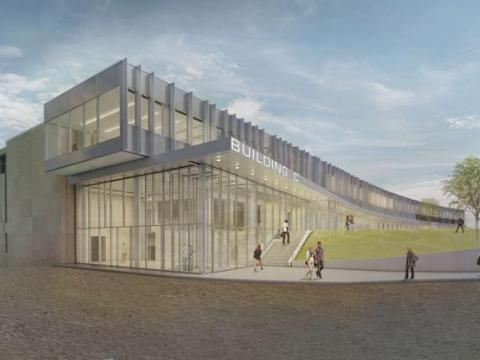
\includegraphics[height=3cm]{briefs-mountaintop-tech-building-initiative.jpg}
\end{center}
%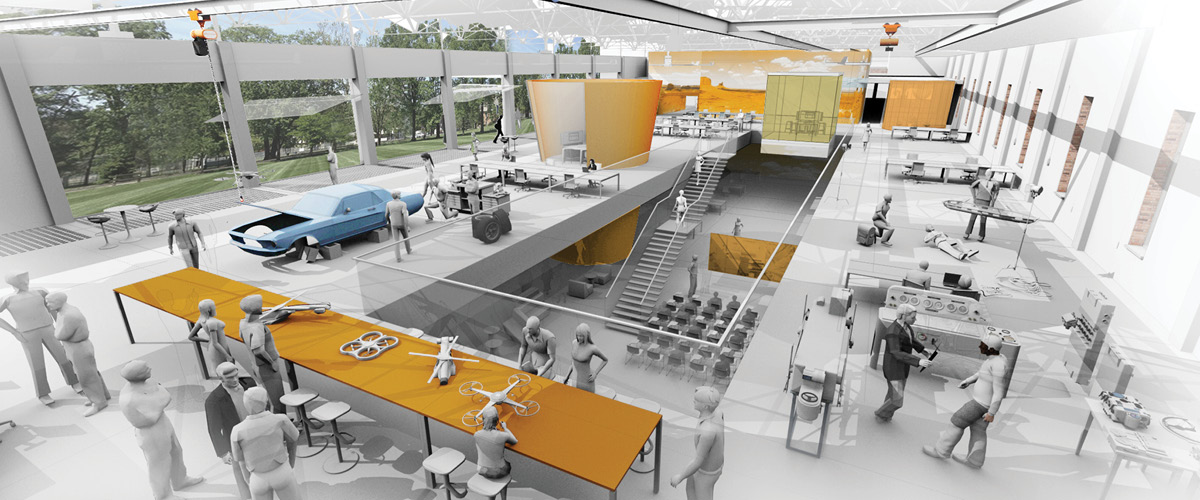
\includegraphics[height=3cm]{Path_to_Prominence_Lehigh_University_Evolution_MountaintopRendering_0.jpg}


\paragraph{The conference facilities} The TRIPODS/DIMACS workshop and the MOPTA conference will be held in Mountain Top Campus is Lehigh's Iacocca Conference Center (\url{https://financeadmin.lehigh.edu/content/iacocca-conference-center}). The building includes dining facilities as well as several breakout and meeting rooms. In particular it main dining room can accommodated up to 300 people, but is ideal setting for a plenary session for about 100-120 participants. Breakout rooms can fit 40-50 people and there is ample space for posters in the foyer leading to the dining room (see the pictures below)
\begin{center}
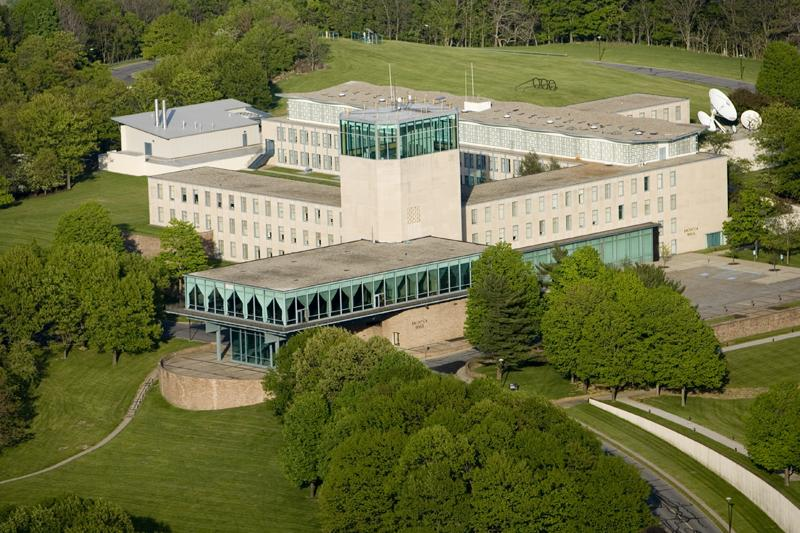
\includegraphics[height=3cm]{Iacocca_Aerial.jpg}
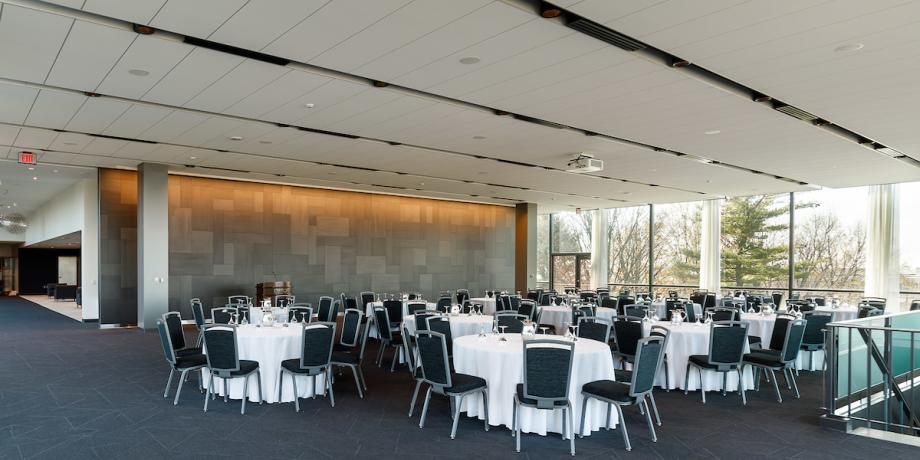
\includegraphics[height=3cm]{wdr.jpg}
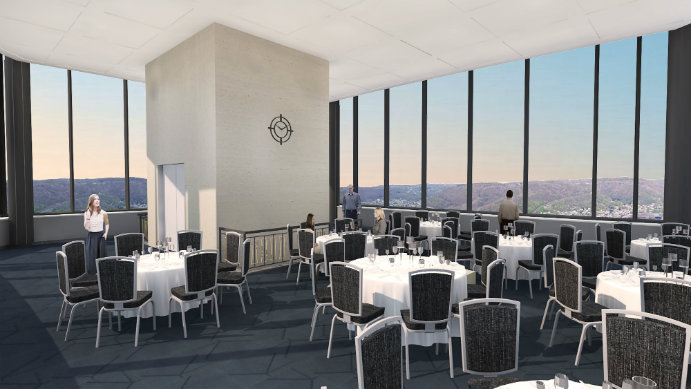
\includegraphics[height=3cm]{Tower_92717.jpg}
%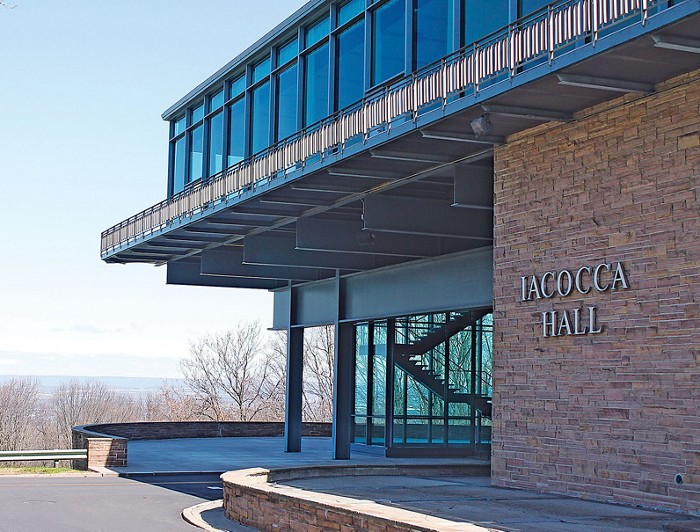
\includegraphics[height=3cm]{asfas.jpeg}



\end{center}




An alternative conference facility on Lehigh's main (lower) campus is Rauch Business center. 

The university also has available conference services staff that helps with planning all phases of the event including catering (\url{https://financeadmin.lehigh.edu/content/conference-services-staff}). The university maintains an up-to-date web page with nearby hotels (\url{http://mylehigh.lehigh.edu/s/1127/interior-hybrid.aspx?sid=1127&gid=1&sitebuilder=1&pgid=8950}). 



Lehigh University is well-positioned to serve as national or international conference site.   A large number of universities and industry research centers are within a few hours drive of Lehigh, meaning that participants could reach the cite cheaply and in little time.  For reference, New York City is only 80~miles and Philadelphia is only 60~miles away from Lehigh, and researchers from Pittsburgh to Baltimore to Upstate New York are also within a few hours driving distance. Newark Liberty International airport  is about 1 hours away.  It is also worthwhile to mention that there are benefits of Lehigh \emph{not} being situated in a large city.  Indeed, the Allentown-Bethlehem-Easton area has an airport within a 10-minute drive from Lehigh, but the area is affordable enough that, e.g., workshop participants can find comfortable lodgings at modest cost, for example the conference hotel for TRIPODS/DIMACS/MOPTA event has a negotiated rate of \$80/night. 



% \paragraph{Lehigh's Flying Machines Coliseum}
%\begin{wrapfigure}{r}{0.35\textwidth}
%\center
%    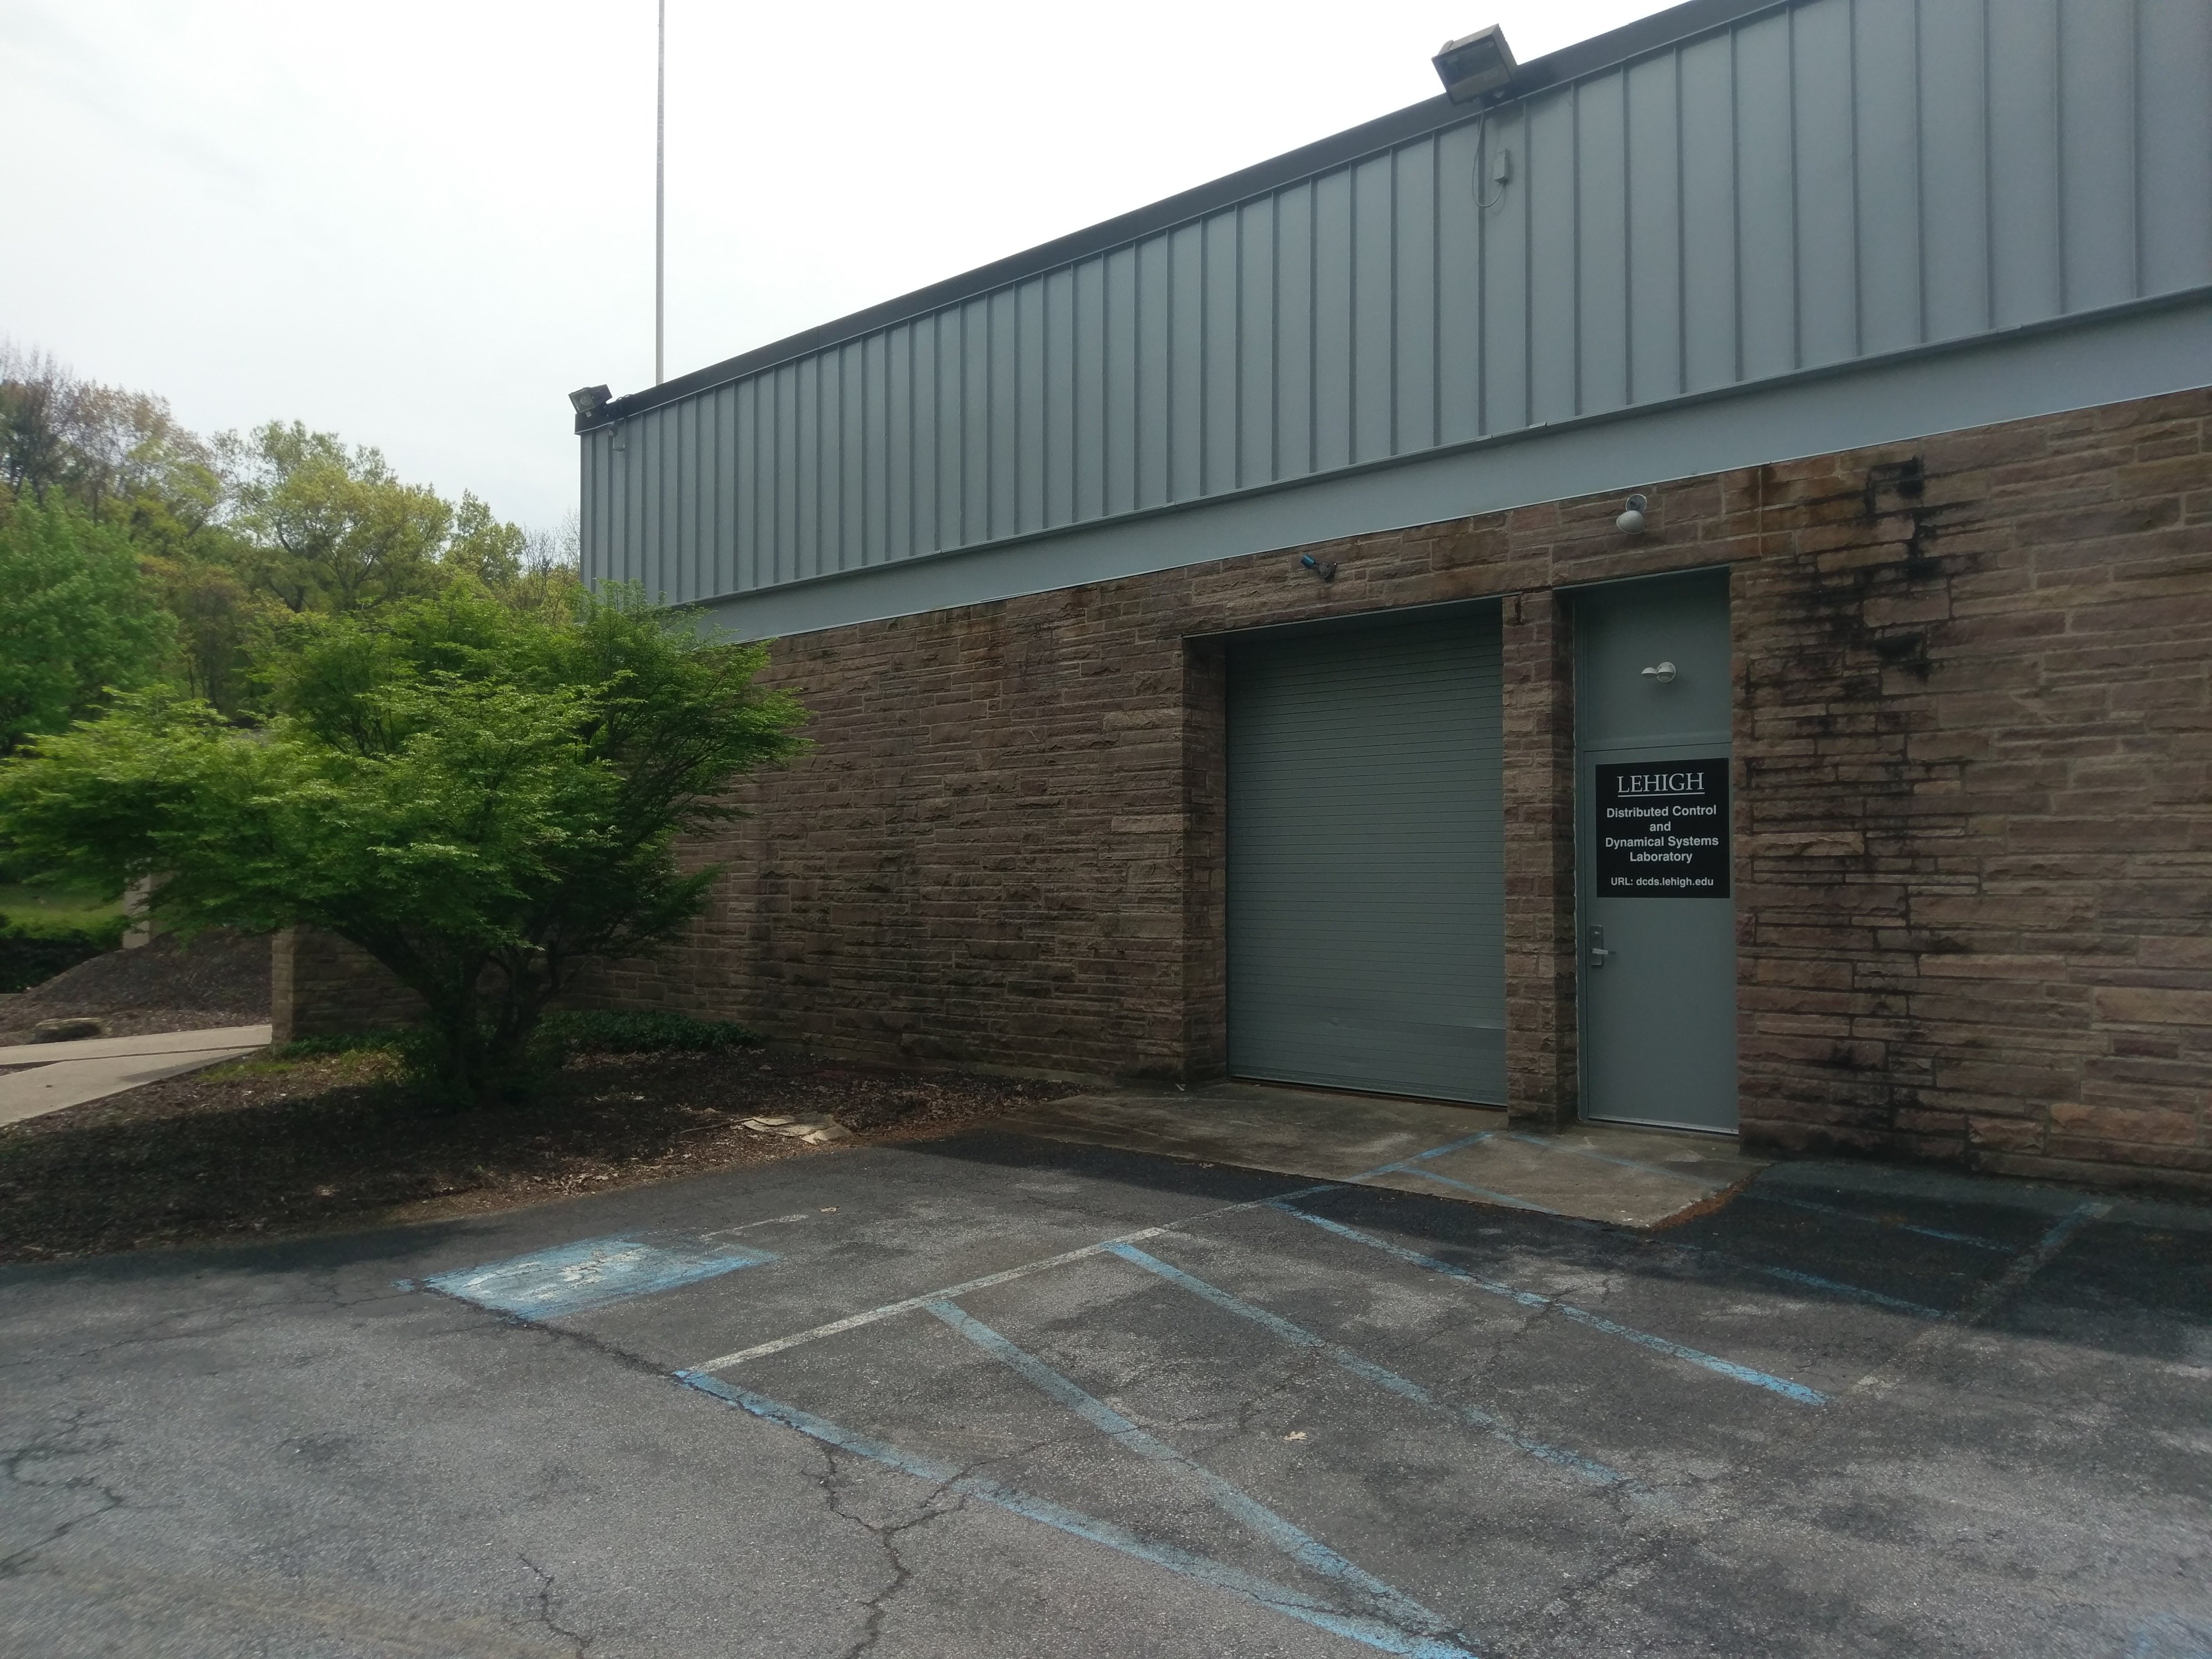
\includegraphics[width=0.35\textwidth]{Facilities/IMAG1065} 
%    \caption*{The LFMC is located at 1515 North Mountain Drive, BETHLEHEM, PA, 18015.}
%\end{wrapfigure}

The summer school for the ML in Robotics workshop  will be implemented in Lehigh's Flying Machines Coliseum (LFMC) which is as part of Distributed Control and Dynamical Systems (DCDS) Laboratory, in the Department of Mechanical Engineering and Mechanics at Lehigh University (see the picture below (left)). 

The mission of LFMC is to investigate experimental aspects of  advanced control capabilities for single or multiple/interconnected quad-copters. The DCDS Lab team is developing design methodologies to optimize drone size, flight controller, and on-board sensors by integrating and co-designing control and navigation algorithms. The group's vision is to unveil the fundamental principles of long-term autonomy.

The LFMC was founded in 2017 as a part of the DCDS group and. Its mission regards experimental research on autonomous flying quad-copters. The overall facility measures up to 4000 square feet and it includes a platform for flying quadcopters, a conference/lab room, an auxiliary office as well as a facility station with a 24/7 running server.

 The main platform covers a space of approximately 3500 square feet. It is equipped with 16 high-precision Opti-Track motion capture system and 4 HD cameras. 
 
% \begin{wrapfigure}{l}{0.35\textwidth} 
%\center
%    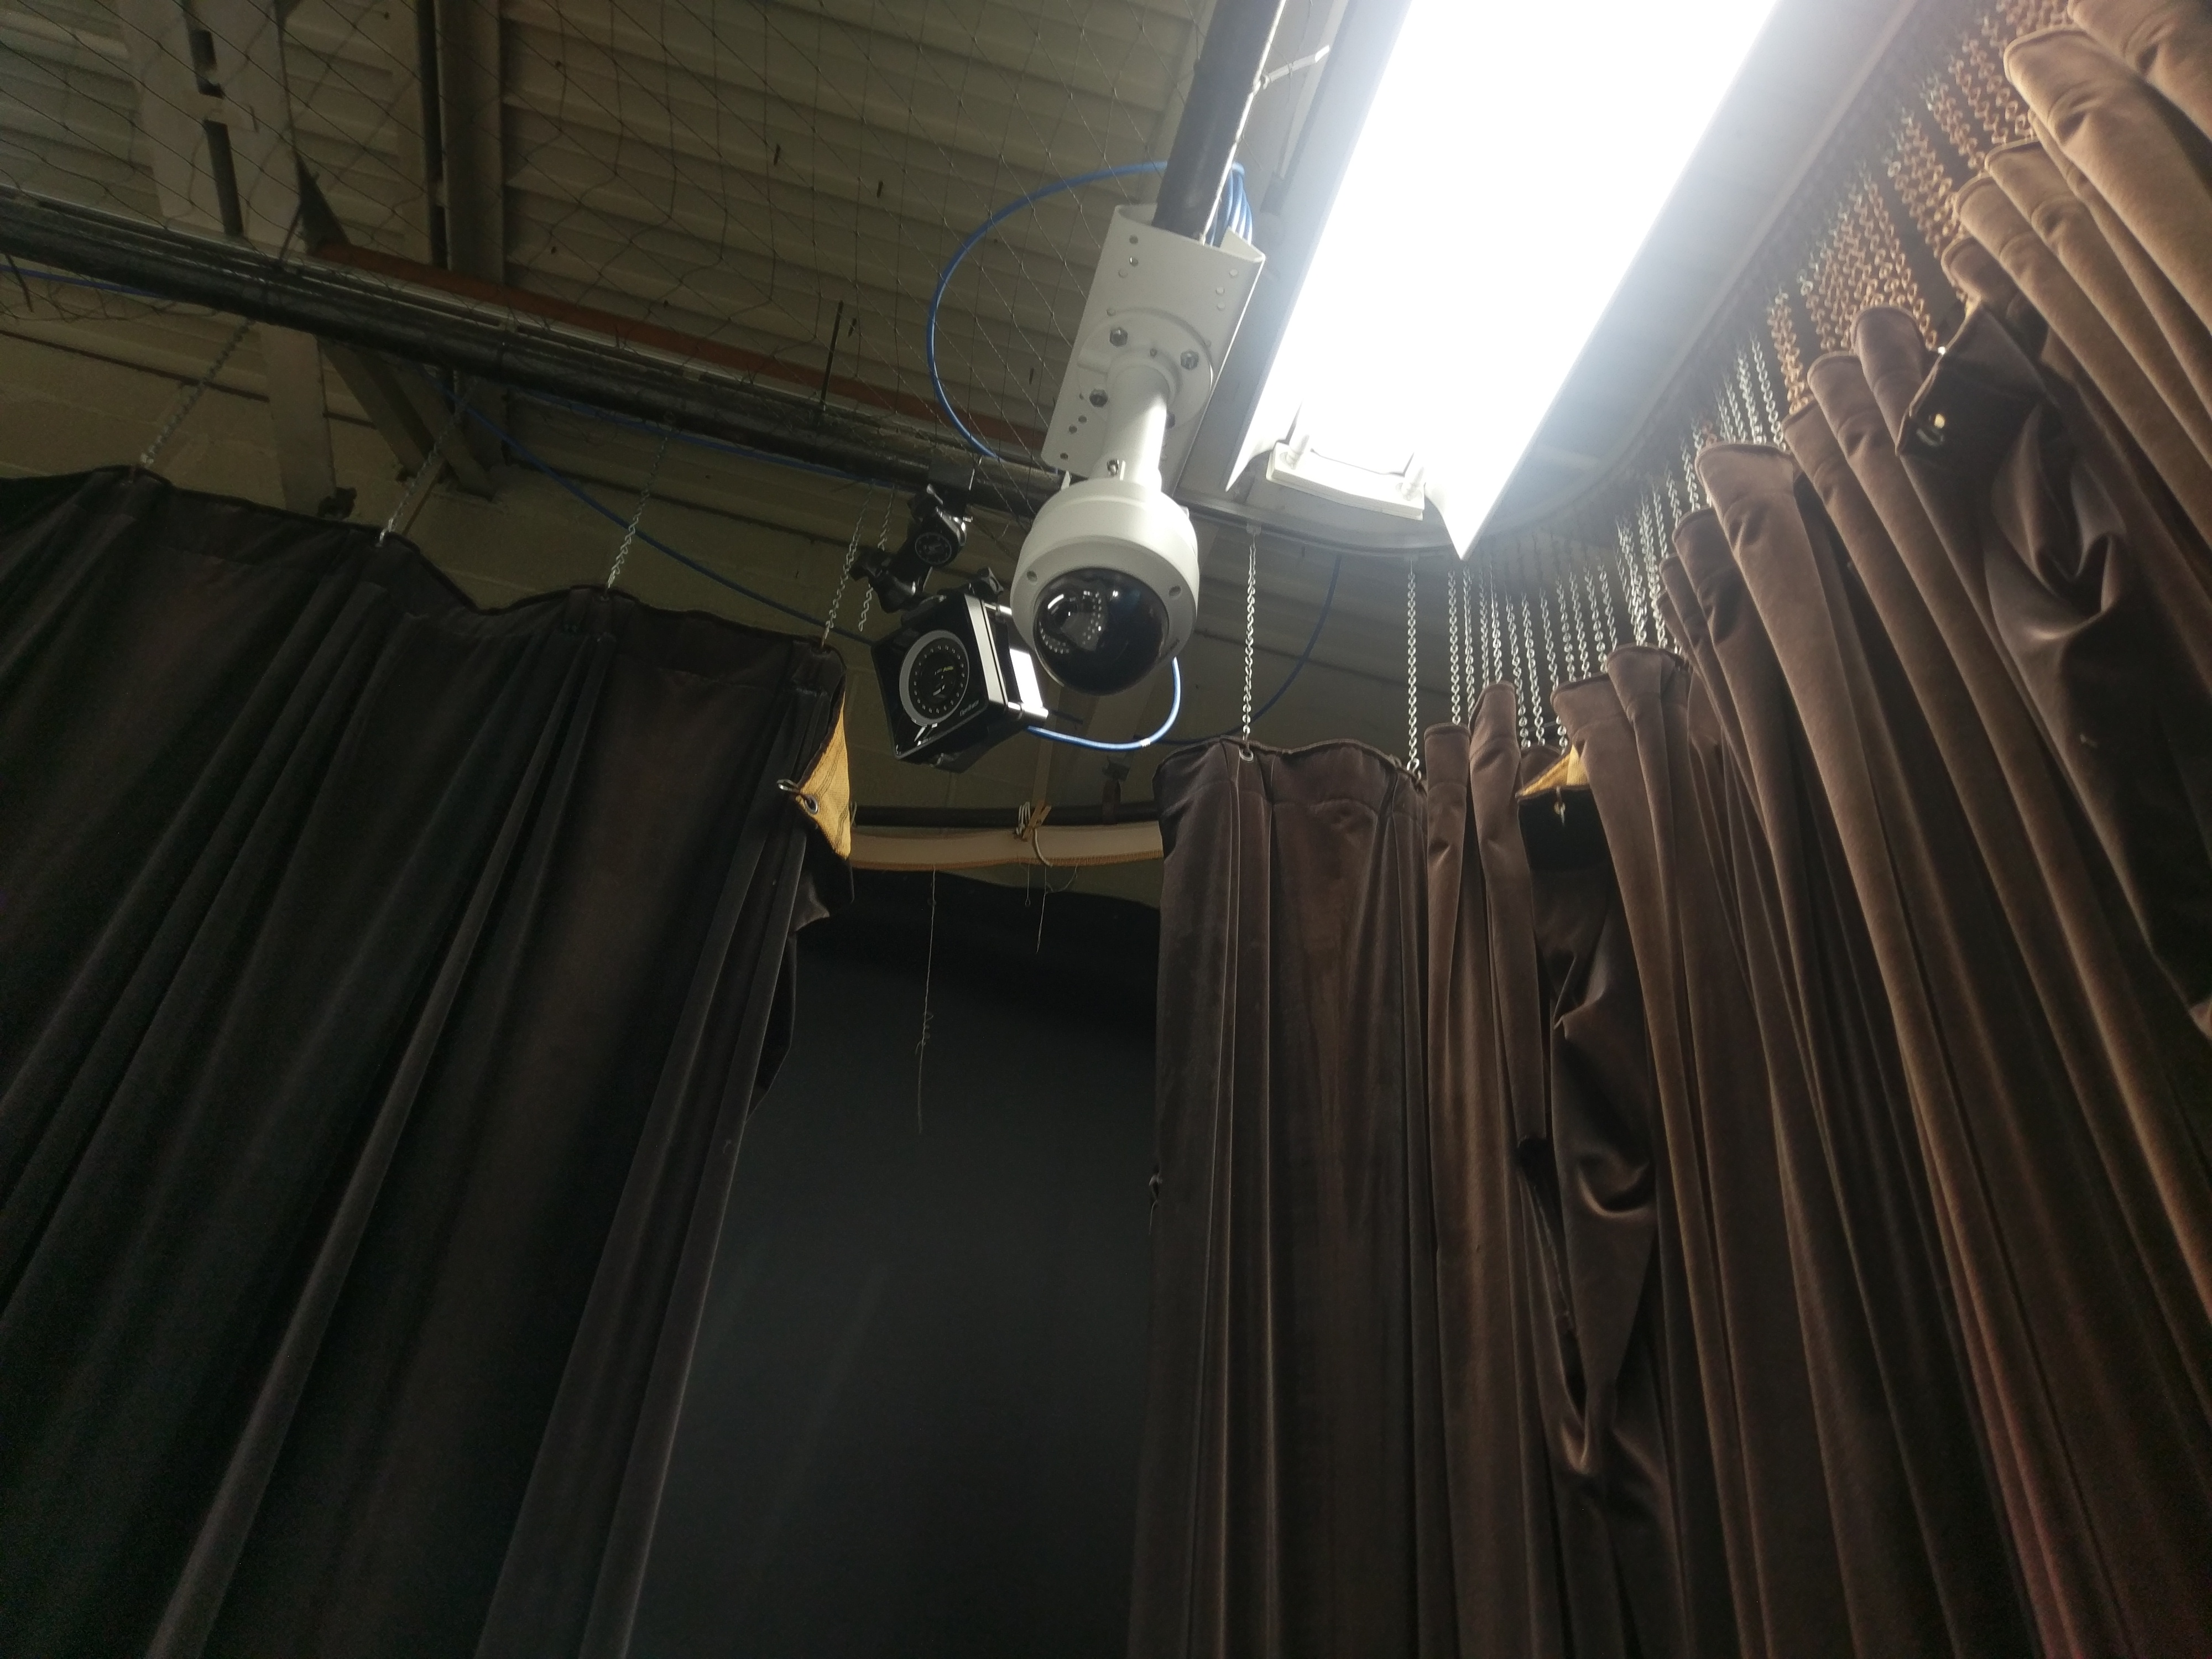
\includegraphics[width=0.35\textwidth]{Facilities/IMAG1089} 
%    \caption*{View of the surveillance system in the Platform room. It consists of the Opti-Track motion capture and the HD camera.}\vspace{-0.5in}
%\end{wrapfigure} 
Real-time experiments are monitored via a high level operating station, that processes motion capture system data to control units using a wireless communication network. The platform space is supported by the server station and the conference/lab room (see the picture below (right)).

 \begin{center}
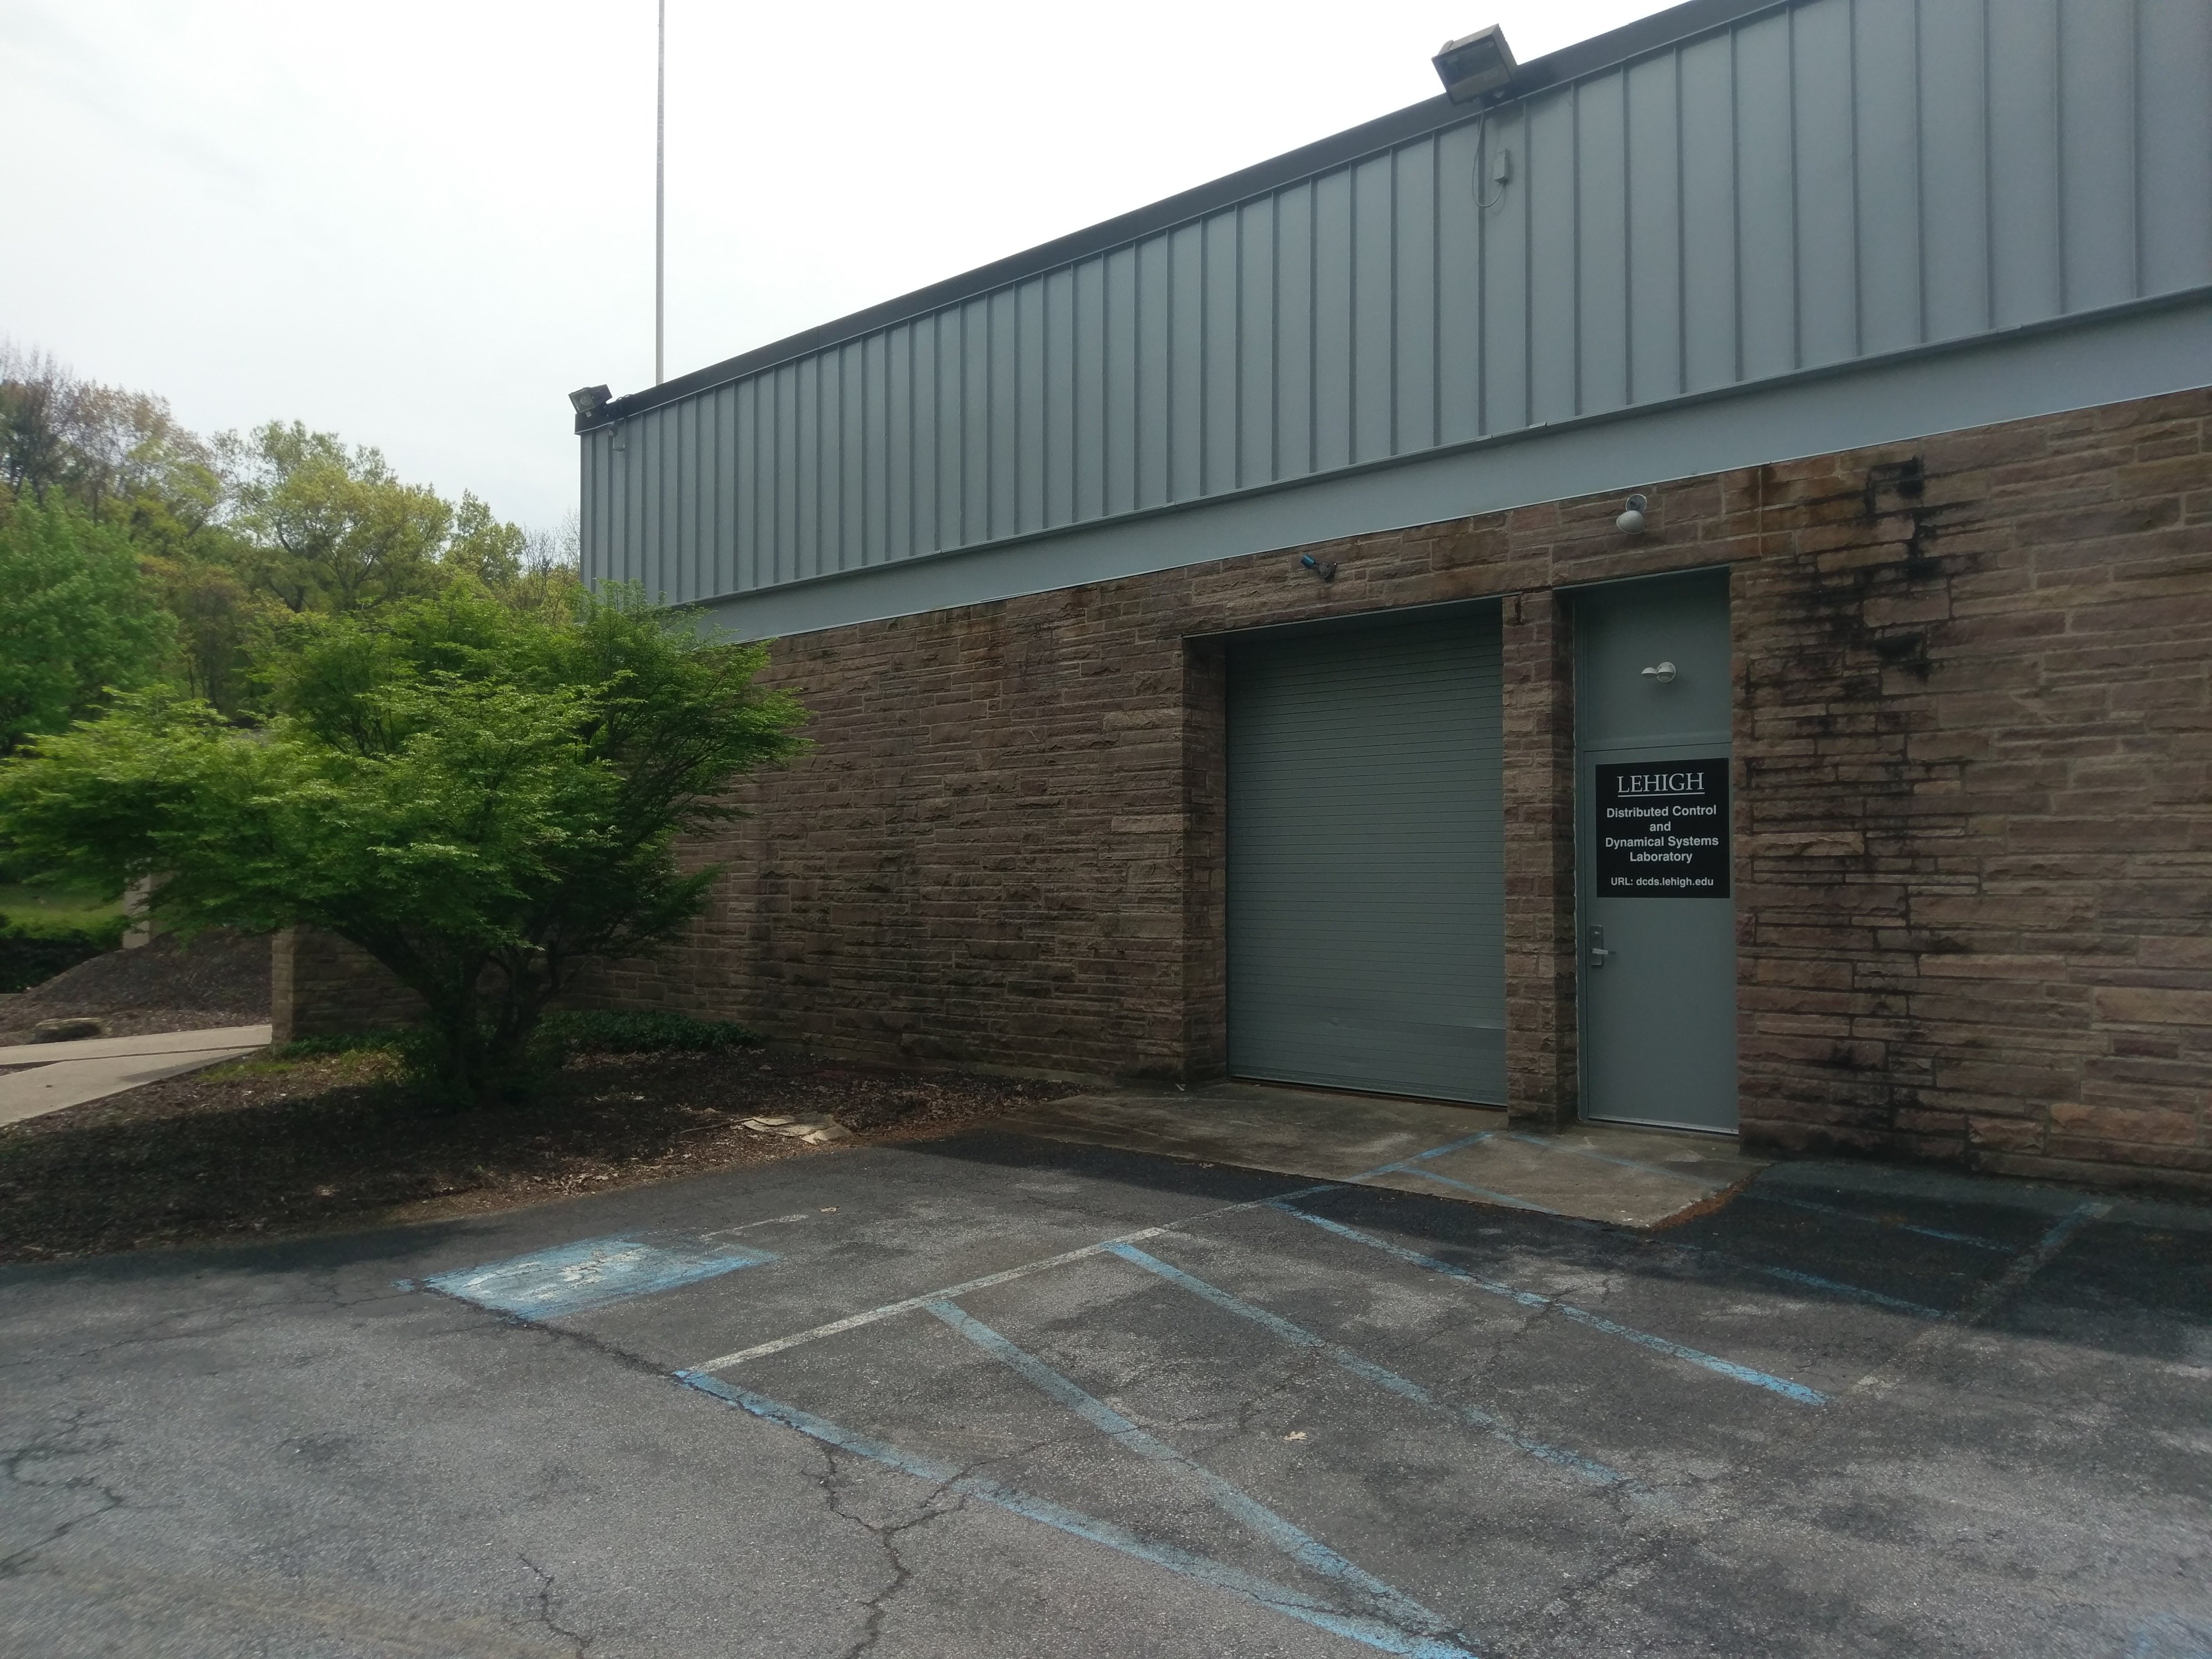
\includegraphics[height=3cm]{Facilities/IMAG1065}
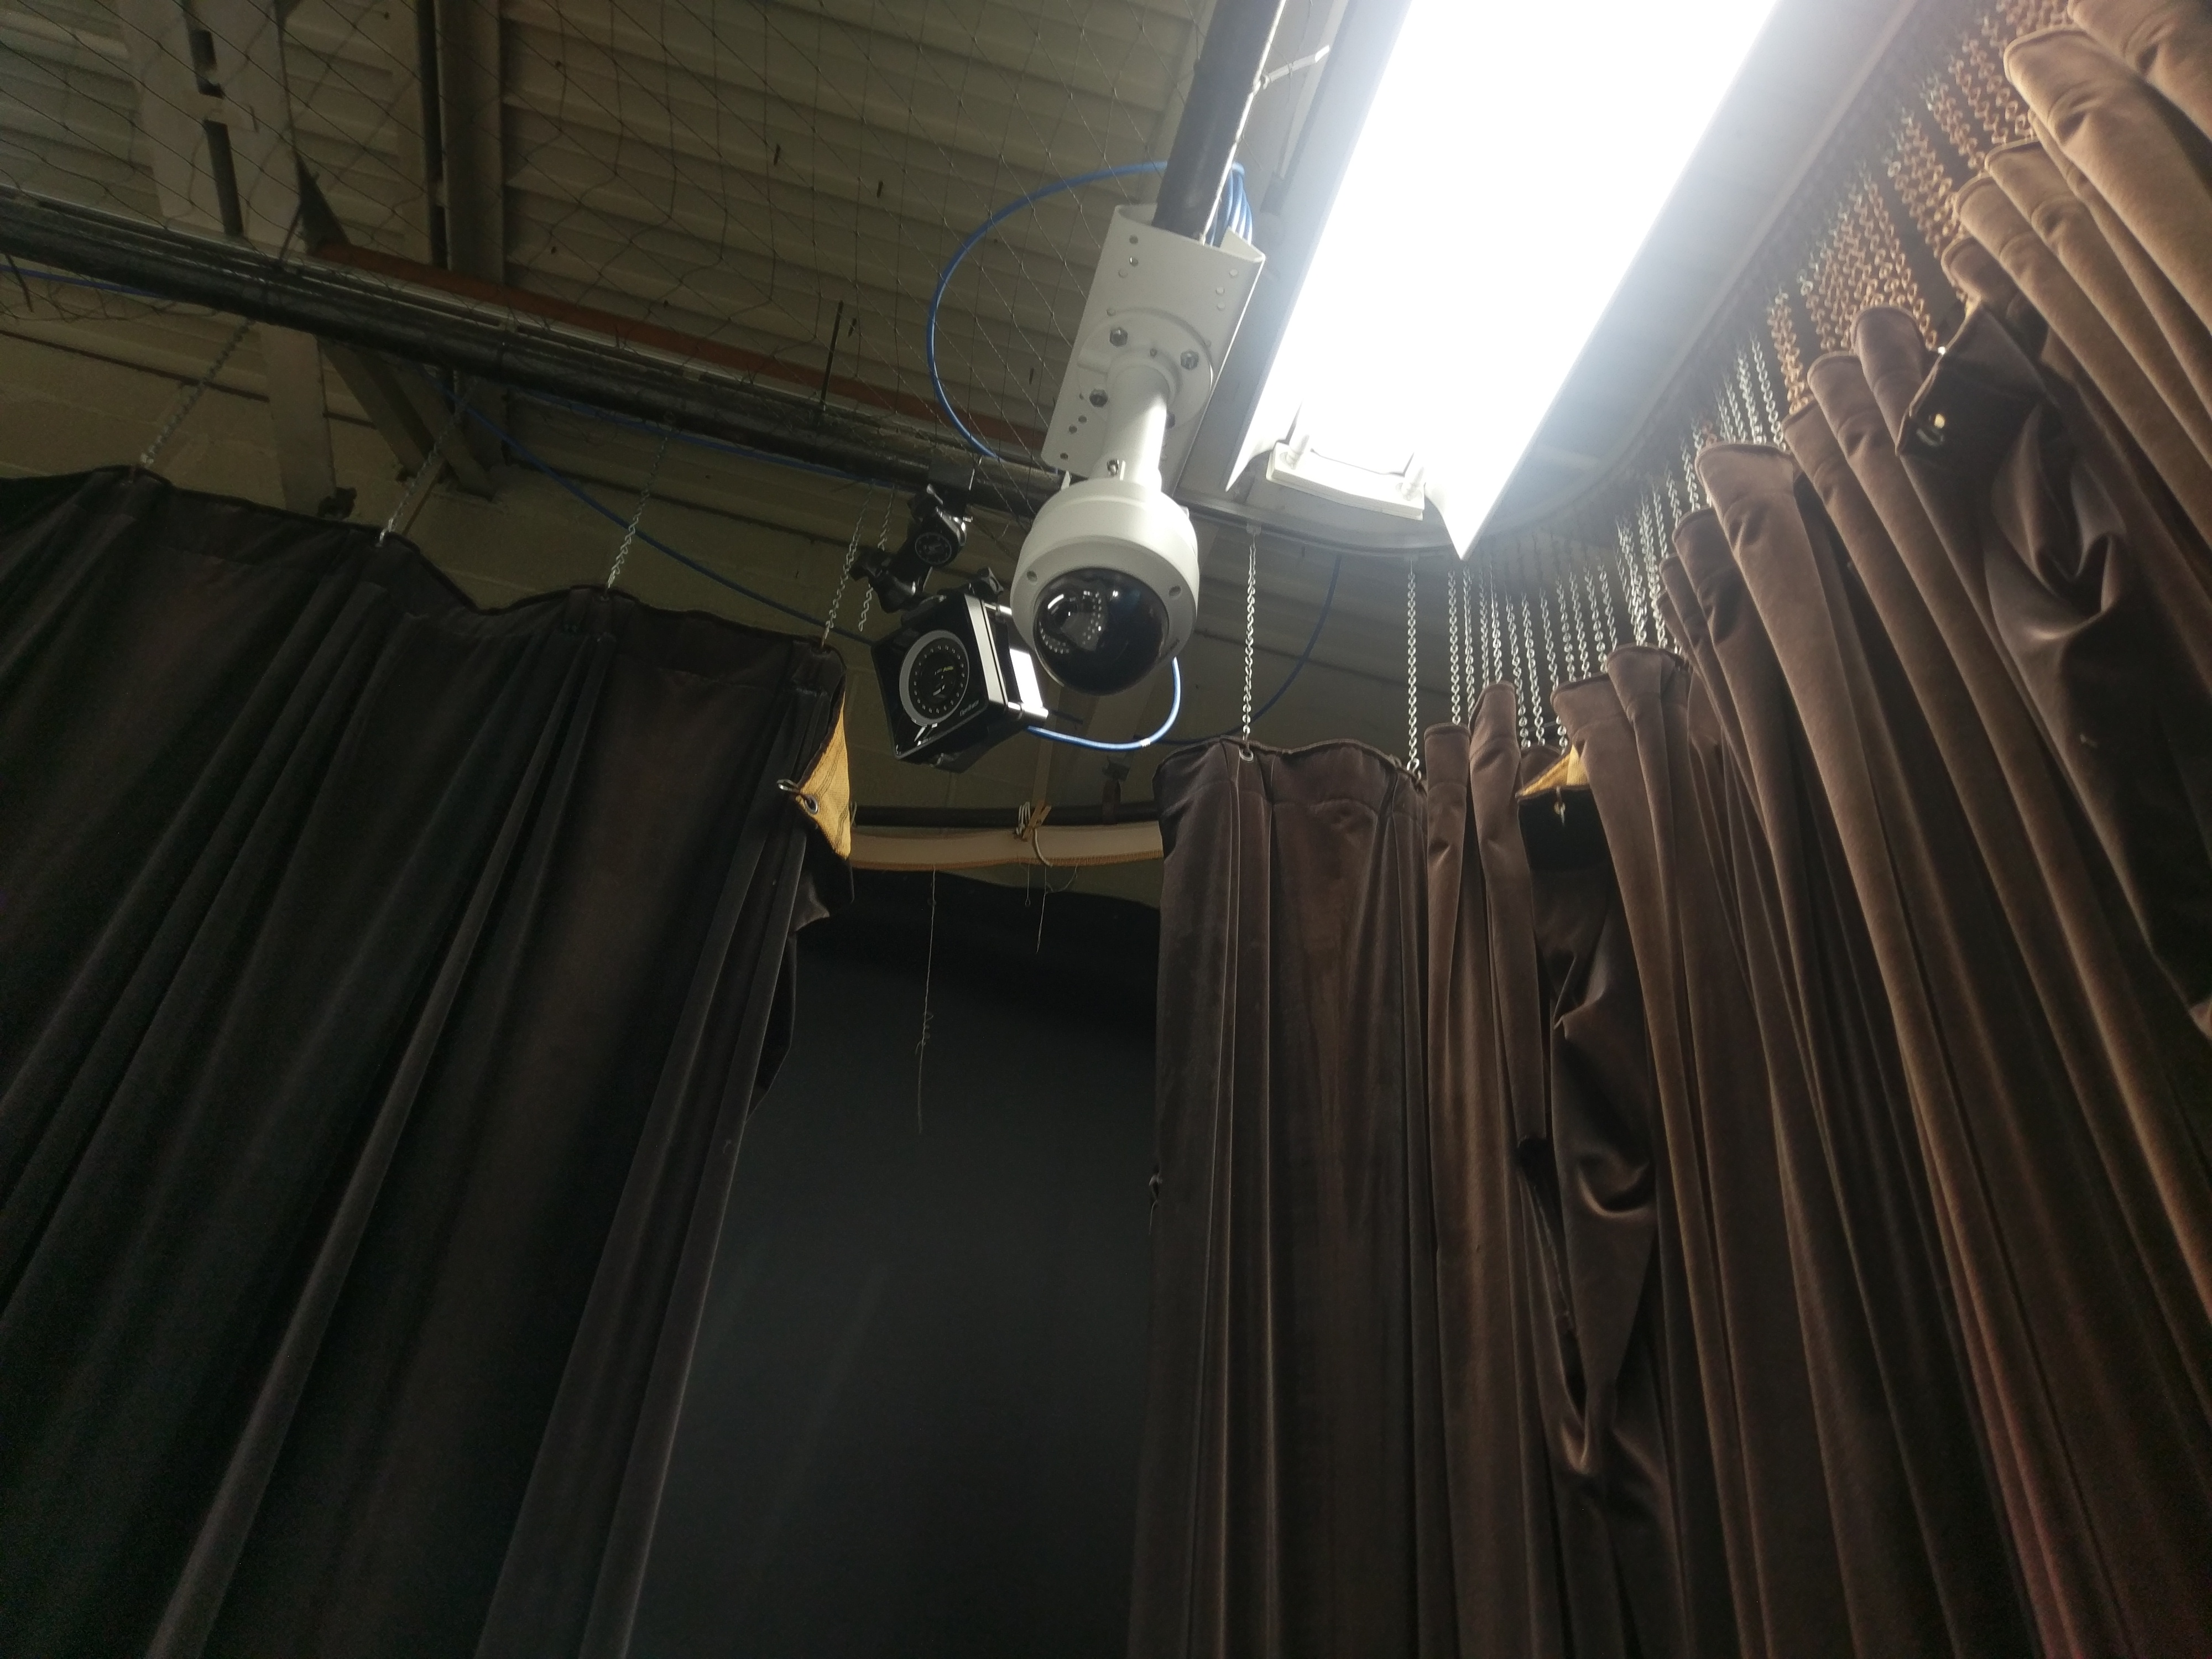
\includegraphics[height=3cm]{Facilities/IMAG1089}

\end{center}




\end{document}
